\item \textbf{{[}DHS/PRELIM/9597/2019/P2/Q1{]} }

The following Gantt chart shows the key tasks involved in a data science
project for a product recommendation engine based on customers' past
purchase patterns.
\noindent \begin{center}
\begin{tabular}{|c|l|c|c|c|c|c|c|c|c|c|c|c|c|c|c|c|c|c|c|c|c|c|}
\hline 
AID & Activity & \multicolumn{21}{c|}{Week}\tabularnewline
\hline 
A & Understand the problem & X & X &  &  &  &  &  &  &  &  &  &  &  &  &  &  &  &  &  &  & \tabularnewline
\hline 
B & Review with team &  &  & X &  &  &  &  &  &  &  &  &  &  &  &  &  &  &  &  &  & \tabularnewline
\hline 
C & Make problem statement &  &  & X &  &  &  &  &  &  &  &  &  &  &  &  &  &  &  &  &  & \tabularnewline
\hline 
D & Define scope of work &  &  & X &  &  &  &  &  &  &  &  &  &  &  &  &  &  &  &  &  & \tabularnewline
\hline 
E & Identify suitable algorithms &  &  &  & X &  &  &  &  &  &  &  &  &  &  &  &  &  &  &  &  & \tabularnewline
\hline 
F & Collect data &  &  & X & X & X & X & X & X &  &  &  &  &  &  &  &  &  &  &  &  & \tabularnewline
\hline 
G & Clean data &  &  & X & X & X & X & X & X &  &  &  &  &  &  &  &  &  &  &  &  & \tabularnewline
\hline 
H & Exploratory data analysis &  &  &  &  & X & X &  &  &  &  &  &  &  &  &  &  &  &  &  &  & \tabularnewline
\hline 
I & Develop use cases &  &  &  &  &  & X & X &  &  &  &  &  &  &  &  &  &  &  &  &  & \tabularnewline
\hline 
J & Present use cases &  &  &  &  &  &  &  & X &  &  &  &  &  &  &  &  &  &  &  &  & \tabularnewline
\hline 
K & Analyse full data &  &  &  &  &  &  &  &  & X & X & X &  &  &  &  &  &  &  &  &  & \tabularnewline
\hline 
L & Develop proof of concept &  &  &  &  &  &  &  &  &  &  &  & X & X & X &  &  &  &  &  &  & \tabularnewline
\hline 
M & Get customer approval &  &  &  &  &  &  &  &  &  &  &  &  &  &  & X &  &  &  &  &  & \tabularnewline
\hline 
N & Build final models &  &  &  &  &  &  &  &  &  &  &  &  &  &  &  & X & X & X &  &  & \tabularnewline
\hline 
O & Deploy models &  &  &  &  &  &  &  &  &  &  &  &  &  &  &  &  &  &  & X & X & \tabularnewline
\hline 
P & Sign off &  &  &  &  &  &  &  &  &  &  &  &  &  &  &  &  &  &  &  &  & X\tabularnewline
\hline 
\end{tabular}
\par\end{center}

A project manager often uses both PERT chart and Gantt chart to illustrate
and manage a project workflow. 
\begin{enumerate}
\item Give one benefit and one limitation of using a Gantt chart to depict
a project workflow?\hfill{} {[}2{]}
\item {}
\begin{enumerate}
\item Construct a PERT chart to depict the project work flow.\hfill{} {[}4{]}
\item State the critical path and the minimum project completion time. \hfill{}{[}2{]}
\item Explain and give an example of a dependent activity.\hfill{} {[}2{]}
\item Explain and give an example of a concurrent activity. \hfill{}{[}2{]}
\item Indicate in your PERT chart and justify a suitable dummy activity.
\hfill{}{[}2{]}
\item Give an example to show your understanding of float or slack time.\hfill{}
{[}2{]}
\end{enumerate}
\item The project manager needs to include a documentation activity and
a cybersecurity activity to the project. Justify the significance
of these activities and show how these can be included in your PERT
chart. Explain any implications to the critical path and projection
completion time. \hfill{}{[}5{]}
\item The project team would inadvertently have access to some restricted
customer purchase information. Give two ethical considerations related
to the privacy of data and suggest possible mitigation measures.\hfill{}
{[}4{]}
\end{enumerate}
The following shows sample interaction snippets of an interactive
exploratory data analysis session. 
\begin{center}
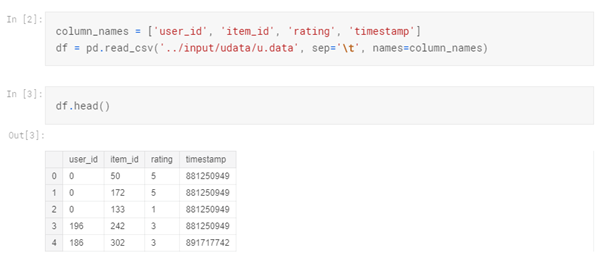
\includegraphics[width=0.65\paperwidth]{C:/Users/Admin/Desktop/Github/question_bank/LyX/static/img/9597-DHS-2019-P2-Q1-1}
\par\end{center}

\begin{center}
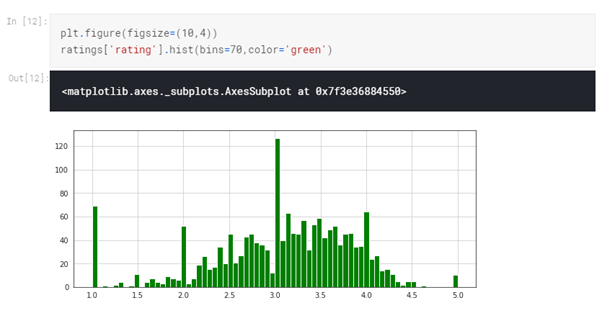
\includegraphics[width=0.65\paperwidth]{C:/Users/Admin/Desktop/Github/question_bank/LyX/static/img/9597-DHS-2019-P2-Q1-2}
\par\end{center}
\begin{enumerate}
\item[(e)]  {}
\begin{enumerate}
\item State the interface used and justify why this is the most appropriate
form of user interaction. \hfill{}{[}3{]}
\item The data analysis team is deciding on whether to perform the analysis
online in a cloud infrastructure or to process all data on a local
computer. What are two factors to consider in arriving at this decision?
\hfill{}{[}2{]}
\item Evaluate the pros and cons of each approach and make a recommendation
with reason(s) to the project team. \hfill{}{[}5{]}
\end{enumerate}
\item[(f)]  Given the relationship: bit rate = baud rate {*} voltage (\# bits
per signal)
\begin{enumerate}
\item Explain the difference between baud rate and bit rate. \hfill{}{[}2{]}
\item The following voltage levels expressed in volts are chosen to encode
bits:

-6.0, -4.5, -3.0, -1.5, +1.5, +3.0, +4.5, +6.0

How many bits represent these voltages?\hfill{} {[}1{]}
\item For the above voltages, write down one possible set of corresponding
bit patterns.\hfill{} {[}1{]}
\item If the baud rate of the line is 900 baud what is the bit rate for
the voltage levels?\hfill{} {[}1{]}
\end{enumerate}